\section{Experiments}
\label{sec:experiments}

We compare our algorithm with \textsc{Banditron} empirically to show that our
kernelized bandit algorithm can have significant advantage over
\textsc{Banditron} in the separable case.

We generated strongly and weakly separable samples with $K=3$ classes shown
in~\autoref{figure:strongly-and-weakly-separable-datasets}. The data sets are
shown as two-dimensional, however, we used a third dimension (so-called
\emph{constant} feature) i.e. a feature that for every example is set to $1$. We
added the constant feature so that \autoref{figure:strongly-separable-dataset}
is actually strongly lineraly separable. For both data sets, the sample size is
$T=5\times 10^6$ and the margin is $\gamma=0.05$.

\begin{figure}[h]
\centering
\begin{subfigure}[b]{0.23\textwidth}
\captionsetup{justification=centering}
\begin{center}
\hspace*{-0.3cm} 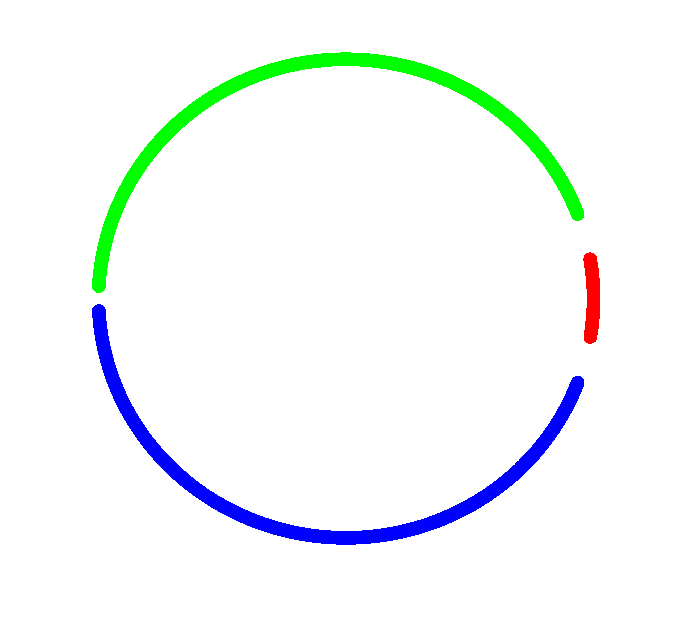
\includegraphics[width=1.15\textwidth, trim={0, 0cm, 0, 0}, clip]{figures/strong_points}
\caption{Strongly separable case}
\label{figure:strongly-separable-dataset}
\end{center}
\end{subfigure}
\hfill
\begin{subfigure}[b]{0.23\textwidth}
\captionsetup{justification=centering}
\centering
\hspace*{-0.3cm}  
\includegraphics[width=1.15\textwidth, trim={0, 0cm, 0, 0}, clip]{figures/weak_points}
\caption{Weakly separable case}
\label{figure:weakly-separable-dataset}
\end{subfigure}
\vspace*{-0.2cm}
\caption{Strongly and weakly generated data sets with $K=3$ classes. All examples lie in
the unit ball. Class 1 is depicted red. Classes 2 and 3 are depcited gree and
blue, respectively. $80\%$ of example belong to class 1, $10\%$ of the data
belong to class 2 and $10\%$ belong to class 3. Class 1 occupies the angle
interval $[-15^\circ, 15^\circ]$, while classes 2 and 3 occupy angle intervals
$[15^\circ, 180^\circ]$ and $[-180^\circ, -15^\circ]$ respectively. We removed
points that lie within margin $\gamma=0.05$ of the linear separators.}
\label{figure:strongly-and-weakly-separable-datasets}
\end{figure}

All results are averaged over $20$ runs.
We plot the number of mistakes against time in Figure~\ref{fig:both}. We can see
there is indeed a dilemma for \textsc{Banditron}: when picking a relatively
large exploration rate, it suffers from the cost of continuous exploration; when
picking a relatively small exploration rate, it cannot adapt its model quickly
enough (this problem exacerbates when a majority class occupies a small region,
like class 1). Striking a balance between the two extremes leads to the
$\sqrt{T}$ mistake bound. On the contrary, our algorithm makes significant
progress on every mistake it makes, leading to a finite mistake bound.

\begin{figure}
    \centering
    \begin{subfigure}[b]{0.23\textwidth}
        \captionsetup{justification=centering}
        \begin{center}
        \hspace*{-0.3cm} 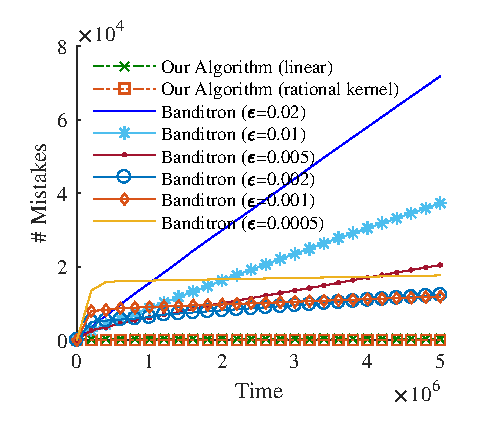
\includegraphics[width=1.15\textwidth, trim={0, 0.1cm, 0, 0}, clip]{figures/strong3}
        \caption{Strongly separable case}
        \end{center}
    \end{subfigure}
    \hfill
    \begin{subfigure}[b]{0.23\textwidth}
        \captionsetup{justification=centering}
        \centering
        \hspace*{-0.3cm}  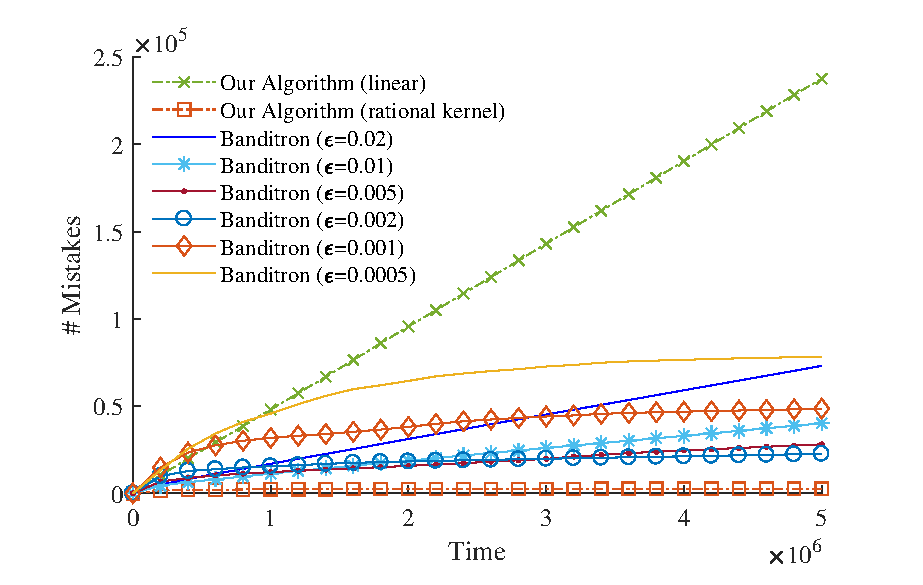
\includegraphics[width=1.15\textwidth, trim={0, 0.1cm, 0, 0}, clip]{figures/weak3}
        \caption{Weakly separable case}
    \end{subfigure}
    \vspace*{-0.2cm}
    \caption{Comparison between our algorithm and Banditron with different exploration parameter $\epsilon$ under $\gamma=0.05$ and $K=3$.}
    \label{fig:both}
\end{figure}
